\documentclass[a4paper]{article}
\usepackage[text={165mm,245mm}]{geometry}
\usepackage{graphicx}
\usepackage{subfigure}
\usepackage{ctex}
\usepackage{float} 
\usepackage{amsmath}
\usepackage{listings}
\usepackage{xcolor}
\definecolor{mygreen}{rgb}{0,0.6,0}  
\definecolor{mygray}{rgb}{0.5,0.5,0.5}  
\definecolor{mymauve}{rgb}{0.58,0,0.82}  
  
\lstset{ %  
  backgroundcolor=\color{white},   % choose the background color; you must add \usepackage{color} or \usepackage{xcolor}  
  basicstyle=\footnotesize,        % the size of the fonts that are used for the code  
  breakatwhitespace=false,         % sets if automatic breaks should only happen at whitespace  
  breaklines=true,                 % sets automatic line breaking  
  captionpos=bl,                    % sets the caption-position to bottom  
  commentstyle=\color{mygreen},    % comment style  
  deletekeywords={...},            % if you want to delete keywords from the given language  
  escapeinside={\%*}{*)},          % if you want to add LaTeX within your code  
  extendedchars=true,              % lets you use non-ASCII characters; for 8-bits encodings only, does not work with UTF-8  
  frame=single,                    % adds a frame around the code  
  keepspaces=true,                 % keeps spaces in text, useful for keeping indentation of code (possibly needs columns=flexible)  
  keywordstyle=\color{blue},       % keyword style  
  %language=Bin,                 % the language of the code  
  morekeywords={*,...},            % if you want to add more keywords to the set  
  numbers=left,                    % where to put the line-numbers; possible values are (none, left, right)  
  numbersep=5pt,                   % how far the line-numbers are from the code  
  numberstyle=\tiny\color{mygray}, % the style that is used for the line-numbers  
  rulecolor=\color{black},         % if not set, the frame-color may be changed on line-breaks within not-black text (e.g. comments (green here))  
  showspaces=false,                % show spaces everywhere adding particular underscores; it overrides 'showstringspaces'  
  showstringspaces=false,          % underline spaces within strings only  
  showtabs=true,                  % show tabs within strings adding particular underscores  
  stepnumber=1,                    % the step between two line-numbers. If it's 1, each line will be numbered  
  stringstyle=\color{orange},     % string literal style  
  tabsize=2,                       % sets default tabsize to 2 spaces  
  %title=myPython.py                   % show the filename of files included with \lstinputlisting; also try caption instead of title  
}  
\title{\heiti 
CODH - 寄存器堆与存储器及其应用 \hspace{0.3cm}实验报告}
\author{院系: \kaishu\underline{}\hspace{1.5cm}姓名: \kaishu \underline{}\hspace{1.5cm}学号: \kaishu \underline{}\hspace{1.5cm}}
\begin{document}
\maketitle

\section{实验目的}
\begin{itemize}
    \item 掌握寄存器堆(Register File)和存储器的功能、时序及其应用
    \item 熟练掌握数据通路和控制器的设计和描述方法
    
    
\end{itemize}

\section{实验环境}
\begin{itemize}
  \item vlab.ustc.edu.cn
  \item Vivado 2016.3
  \item Nexys 4 DDR 开发板
\end{itemize}
\section{实验内容}
\subsection{完成32x32位的寄存器堆的功能仿真}
\begin{itemize}
  \item 端口:ra1, rd1, ra2, rd2, wa, wd, we, clk
  \item 寄存器堆的0号寄存器内容恒定为零
  \item 寄存器堆的写优先的读操作模式
  
\end{itemize}

\subsection{完成排序模块(SRT)的逻辑设计和功能仿真}
\begin{itemize}
    \item 端口:clk, rstn, run, done, cycles, addr, dout, din, we, clk\_ld
    \item 存储器0号位置存放的是待排序数组的长度
    \item 需要注意与SDU的整合端口
  \end{itemize}
  
之后将其与串行调试单元模块(SDU\_DM)整合后,下载至FPGA中测试。

\section{逻辑设计 / 核心代码}
\subsection{32x32位的寄存器堆}
\subsubsection{逻辑设计}
只需更改ppt中提供的代码即可,添加时序逻辑使0号寄存器的内容恒定为零。

至于写优先的读操作模式,由于此处由组合逻辑实现(读的永远是寄存器的最新值),不需要特别设置。但为了之后的实验还是加入了相关判断语句。
\subsubsection{核心代码}
\begin{lstlisting}[language={verilog},title={reg.v}] 
  reg [DWidth - 1:0]  rf [0: (1 << AWidth) - 1]; 	//寄存器堆

  always@(ra1, ra2)
      rf[0] = 0;
  
  always  @(posedge  clk)
  begin
      if (we && wa != 0)  rf[wa]  <=  wd;   //写操作
  end
  
  assign rd1 = (ra1 == wa && we == 1 && wa != 0) ? wd : rf[ra1];  //写优先的读操作1
  assign rd2 = (ra2 == wa && we == 1 && wa != 0) ? wd : rf[ra2];  //写优先的读操作2
\end{lstlisting}

\subsubsection{模块仿真}
直接对默认的32x32 REG 进行仿真,编写了相应的test bench进行测试,
在 Vivado 仿真后得到波形图:
\begin{figure}[H]
    \centering
    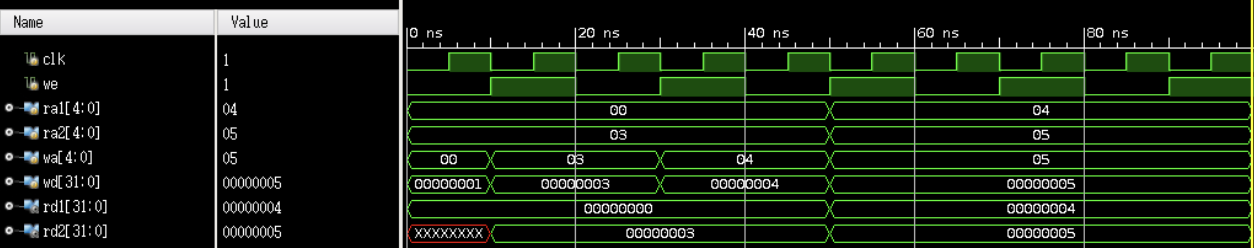
\includegraphics[width=1.0\textwidth]{reg_sim.png}
    \caption{REG SIM波形图}
    \label{fig:reg_sim}
  \end{figure}

可以看到0号寄存器的内容恒定为零,写优先的读操作模式也正确。

\subsection{排序(SRT)}
\subsubsection{逻辑设计}
一开始不考虑与SDU的整合,只考虑排序模块的逻辑设计,并将使用SDU的调试读写阶段预先留出。

我们采用冒泡排序,先用高级语言写出后参照结构更改为FSM:
\begin{lstlisting}[language={verilog},title={sort.c}]
    for (int i = 1; i <= n - 1; i++)
        for (int j = 1; j <= n - i + 1; j++)
        if(M[j] > M[j+1]) 
            { temp = M[j];  M[j] = M[j+1]; M[j+1] = temp; }
\end{lstlisting}

由此可以画出以下状态转换图。

\begin{figure}[H]
    \centering
    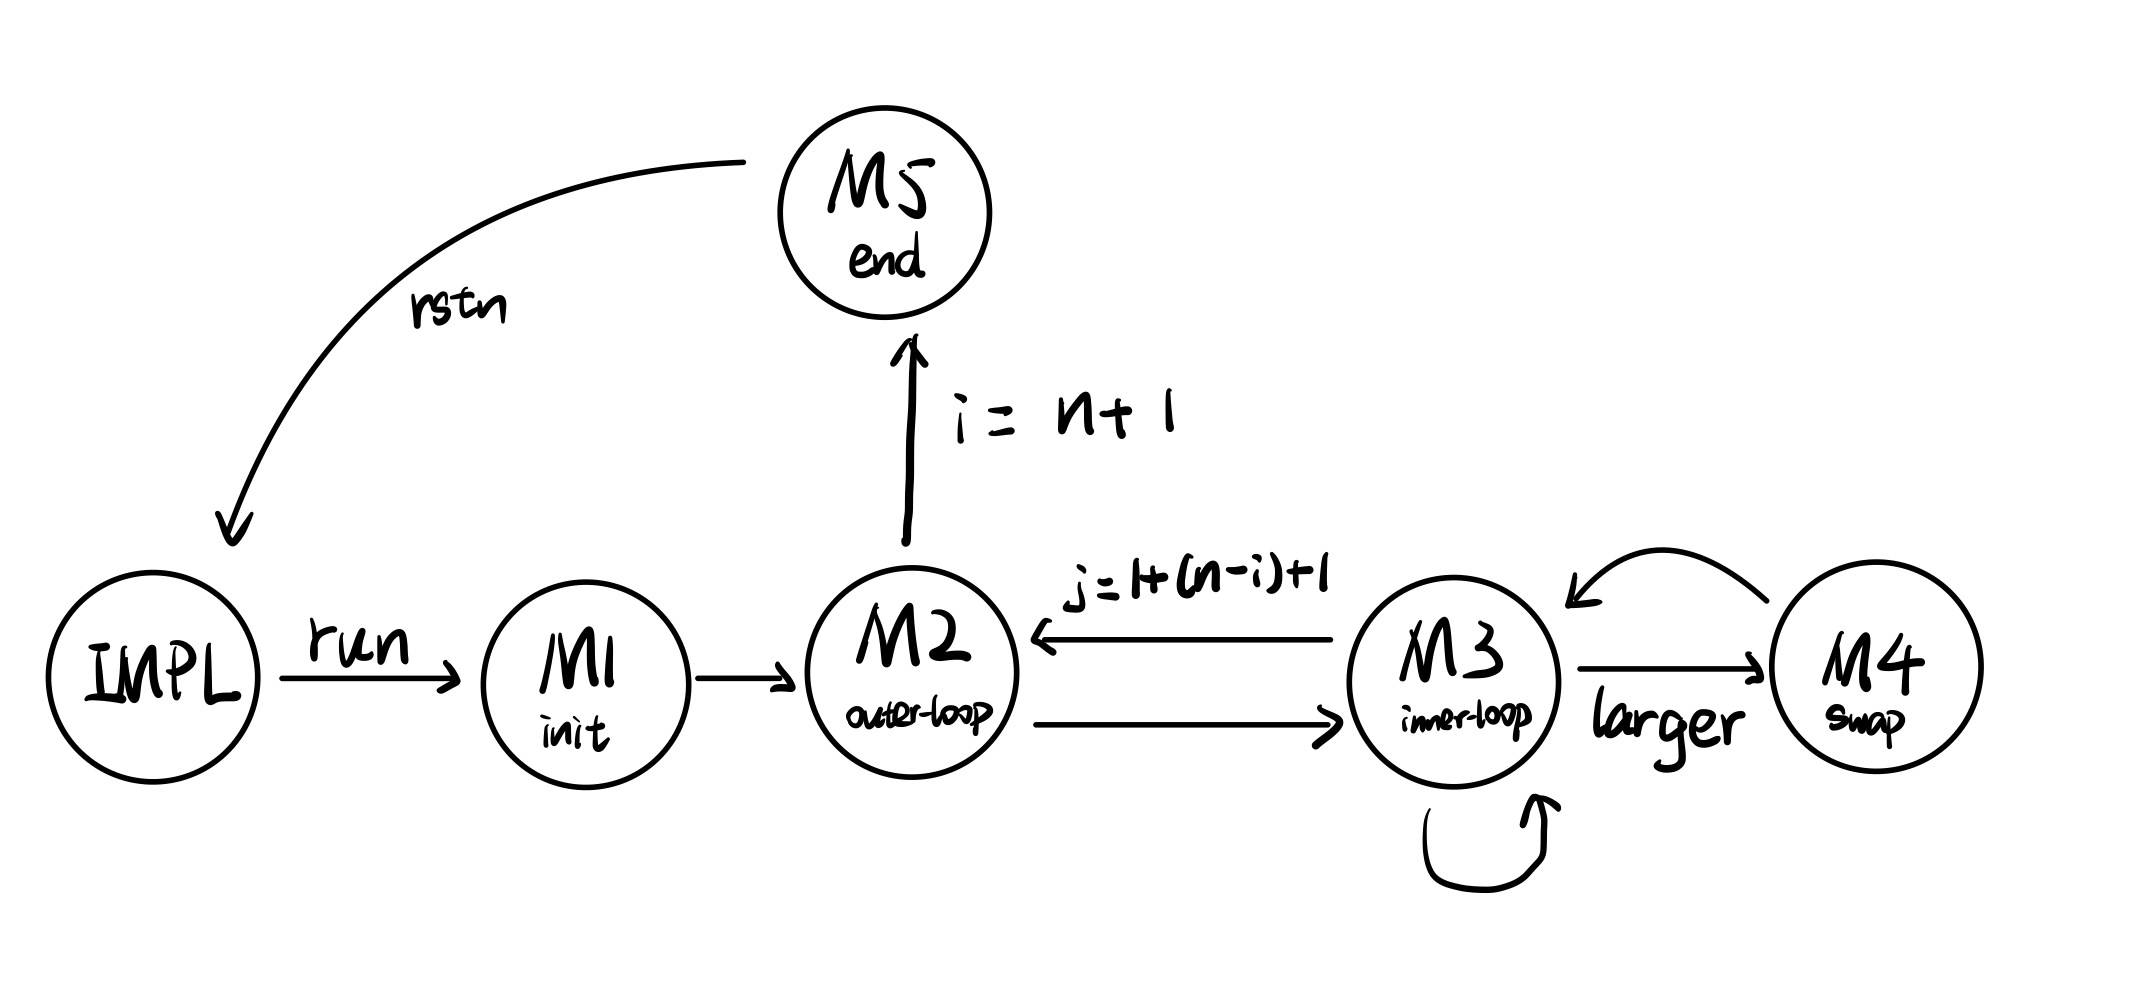
\includegraphics[width=0.9\textwidth]{fsm.jpeg}
    \caption{状态转换图}
    \label{fig:fsm}
  \end{figure}

IMPL 状态为默认状态,当复位信号有效时恢复到此状态,此时存储器的各信号切换为SDU输入的信号,可以使用SDU查看或设置存储器中的内容。

当按下按钮,run信号有效,状态机切换至状态M1状态,在此状态做一些进入循环前的参数准备,例如将存储器的各型号切换为SRT内部信号。

接着切换至M2状态,此状态负责检查外层循环是否达到终止条件以及内层循环的参数设置(若i = n + 1,下一步进入结束状态M5)。

否则M2切换到M3,进行内层循环,此状态负责检查内层循环是否达到终止条件以及比较相邻两个数的大小并交换(若j = n - i + 2,下一步进入M2,进行下一循环;
若M[j] > M[j+1],设置写入信号将M[j]设为M[j+1],temp存为M[j],然后切换到M4状态进行另一半切换)。

对于M4状态,设置写入信号将M[j+1]设为temp(M[j]),然后切换回M3状态进行下一次内层循环。

对于M5结束状态,将存储器的各信号切换为SDU输入的信号,并且保持cycle信号不变显示状态数。若要进行下一次排序,通过按下rstn切换为IMPL再按下run即可。

\subsubsection{核心代码}
flag 信号用于切换来自SDU的信号还是SRT内部的信号。 由于每次读相邻两个存储器的内容,因此将dpra端口链接为a+1。
由于在下一个时钟边沿到来时才会更新存储器的内容,为了实现写优先,设置了real\_spo来标识写优先模式下读出的存储器内容。
larger信号则是由组合逻辑实现的比较相邻两个数的大小,若M[j] > M[j+1],则larger为1,否则为0。

具体信号数据设计参见代码及注释。
\begin{lstlisting}[language={verilog},title={srt.v}]
    ...
    // 次态切换
    always@(*) begin
    ns = cs;
    case (cs)
        IDLE: begin
            if (run) begin
                ns = M1;
            end
        end
        M1:
            ns = M2;
        M2: begin
            if (i == n + 1 | ~swaped)
                ns = M5;
            else
                ns = M3;
        end
        M3: begin
            if (a == n - i + 2)
                ns = M2;
            else if (larger)
                ns = M4;
            else
                ns = M3;
        end
        M4: begin
            ns = M3;
        end
        M5: begin   //finish, display cycles
            ns = M5;
        end
    endcase
    end

    assign dpra = a + 1; //dpra = j+1, a = j, spo=M[j], dpo=M[j+1]
    assign real_spo = we_srt ? d : spo;  //write first
    assign larger = (real_spo <= dpo) ? 0 : 1; //larger -> swap
    //组合逻辑设置信号
    always@(posedge clk or negedge rstn)
    begin
    if(~rstn)
    begin // default state for sdu
        a <= 0; //For MEM[0]
        finish <= 1;
        swaped <= 0;
        flag <= 0;
        cnt <= 0;
        n <= 0;
        i <= 1;
        cnt <= 0;
        we_srt <= 0;
        temp <= 0;
        d <= 0;
    end
    else
    case (cs)
    IDLE: begin // default state for sdu
        a <= 0; //For MEM[0]
        finish <= 1;
        swaped <= 0;
        flag <= 0;
        cnt <= 0;
        n <= 0;
        i <= 1;
        cnt <= 0;
        we_srt <= 0;
        temp <= 0;
        d <= 0;
    end

    M1: begin // init
        finish <= 0;
        n <= spo;
        i <= 1;
        swaped <= 1;
        flag <= 1;
        cnt <= cnt + 1;
    end

    M2: begin // outer-loop
        we_srt <= 0;
        a <= 1;
        swaped <= 0;
        cnt <= cnt + 1;
    end

    M3: begin // inner-loop
        if(a != n - i + 2 && larger) begin //-> M4 -> M3 to swap, M[j] = M[j+1], temp = M[j]
            swaped <= 1;
            d <= dpo;
            we_srt <= 1;
            temp <= real_spo;
        end
        else if(a == n - i + 2)begin // -> M2
            a <= 1; //a = j =1 
            we_srt <= 0;
            i <= i + 1; //i = i + 1
            swaped <= 1;
        end
        else begin //-> M4, a = j = j + 1
            we_srt <= 0;
            a <= a + 1;
        end
        cnt <= cnt + 1;
    end

    M4: begin //swap
        a <= a + 1; // M[j+1] = temp = M[j], j = j + 1
        d <= temp;
        we_srt <= 1;
        cnt <= cnt + 1;
    end

    M5: begin //end
        finish <= 1;
        flag <= 0;
    end

    endcase
    end
\end{lstlisting}
\subsubsection{模块仿真} 
将ip核使用coe文件初始化内部数据为 x10, xf, xe, xd, xc, xb, xa, x9, x8, x7, x6, x5, x4, x3, x2, x1, x0.
然后编写调用srt模块的testbench,在Vivado进行仿真,测试结果如下(最终存储器内数据) 
\begin{figure}[H]
    \centering
    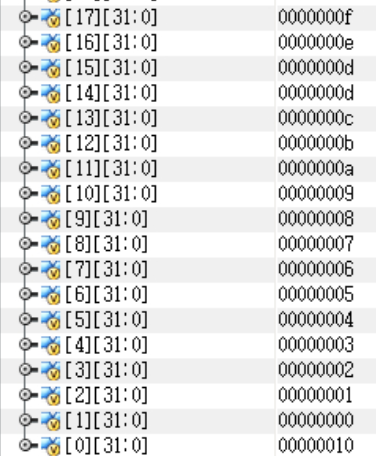
\includegraphics[width=0.5\textwidth]{srt_sim.png}
    \caption{SRT SIM结果图}
    \label{fig:srt_sim}
  \end{figure}

可以发现SRT模块很好地完成了任务,将16个数字排序成了升序。

\subsubsection{下载测试}
首先需要编写取边沿,去抖动的模块,对run进行处理:
\begin{lstlisting}[language={verilog},title={edge.v}]
  ...
  always@(posedge clk)
    begin
        if (en == 0)
            cnt <= 0;
        else if (cnt < 16'h8000)
            cnt <= cnt + 1;
        en1 <= cnt[15];
        en2 <= en1;
    end
  assign out = en1 & ~en2;
\end{lstlisting}
然后编写top模块,并将SDU整合进去(只需将SDU相应的输出信号接入SRT对应的输入信号即可)。同时为了更直观的看到结果,用16位LED作为cycles的输出。
其余显示并不必要,因为SDU可以方便的查看及改变存储器的内存数据

\begin{lstlisting}[language={verilog},title={top.v}]
    sort_with_sdu srt_inst(
        .clk(clk),
        .rstn(rstn),
        .run(out),
        .done(done),
        .cycles(cycles),
        .addr(addr),
        .dout(dout),
        .din(din),
        .we(we),
        .clk_ld(clk_ld) 
    );
        
    sdu_dm sdu_inst(
        .clk(clk),
        .rstn(rstn),
        .rxd(rxd),
        .txd(txd),
        .addr(addr),
        .dout(dout),
        .din(din),
        .we(we),
        .clk_ld(clk_ld)
    );

\end{lstlisting}

然后生成bit流进行烧写测试。一开始由于生成速度过慢导致难以发现某些错误,因此降低了时钟频率。最终在助教的帮助下发现了top模块内实例化的srt未加入din端口,这导致了大部分错误,将其改正后程序正确运行且通过了检查。

随机输入数据进行测试,结果如下图所示:
\begin{figure}[H]
    \centering
    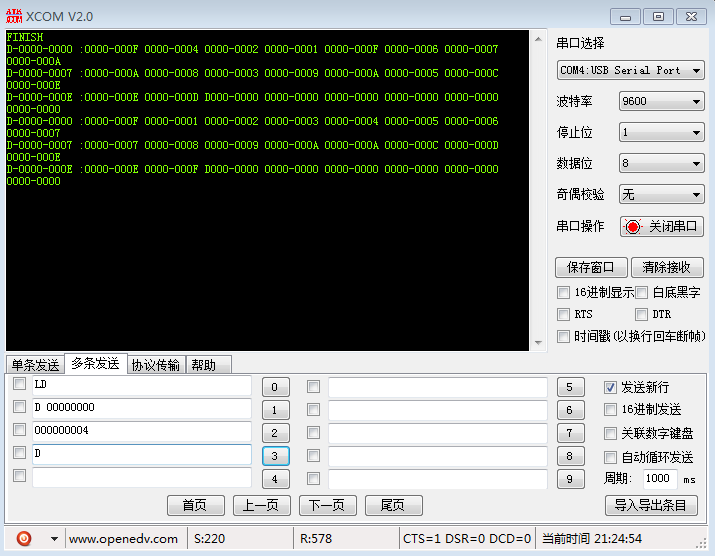
\includegraphics[width=0.9\textwidth]{top.png}
    \caption{实际结果图}
    \label{fig:top}
  \end{figure}

\subsubsection{结果分析}
RTL电路:
\begin{figure}[H]
    \centering
    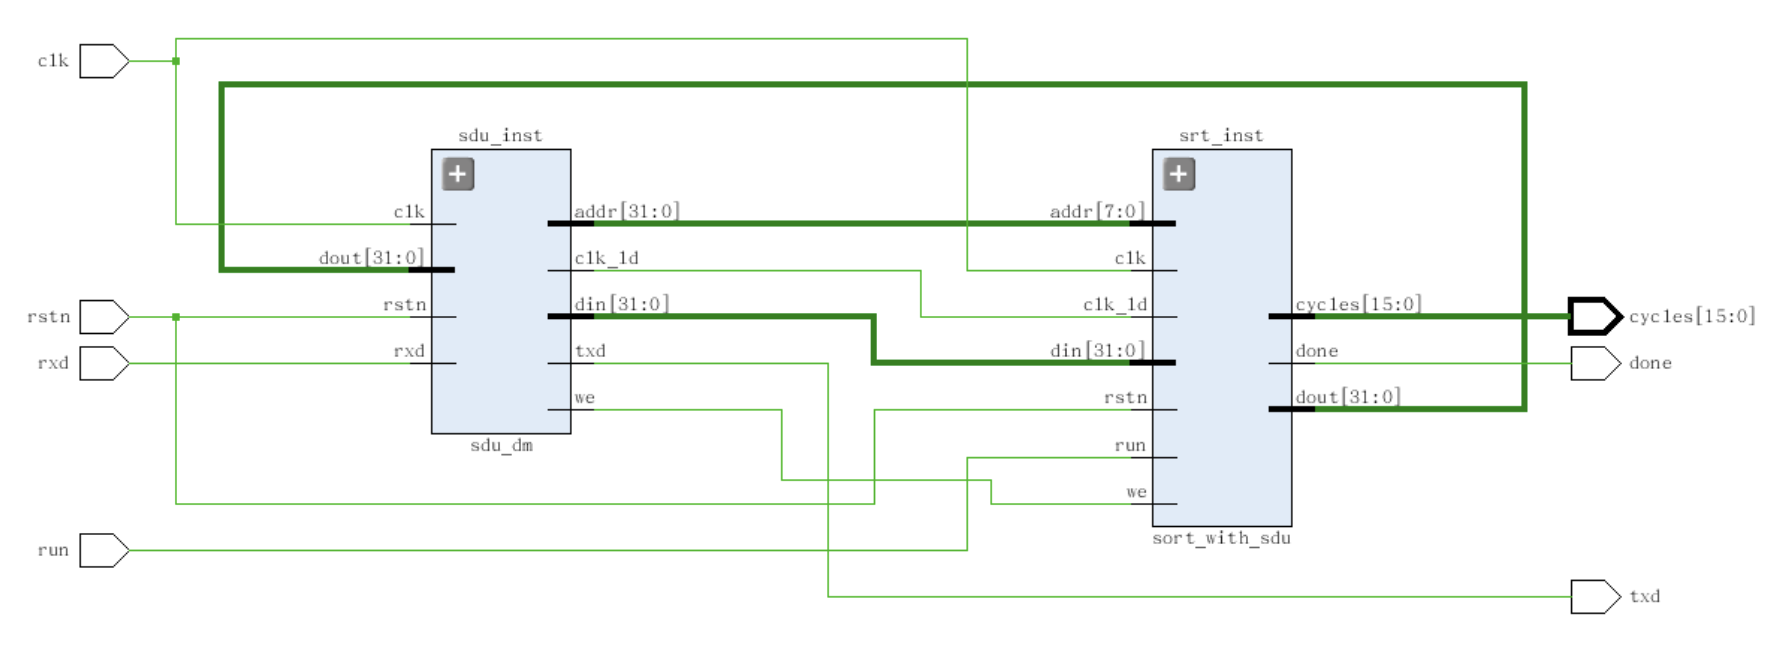
\includegraphics[width=1.0\textwidth]{rtl.png}
    \caption{RTL}
    \label{fig:rtl}
  \end{figure}


电路资源使用情况:
\begin{figure}[H]
    \centering
    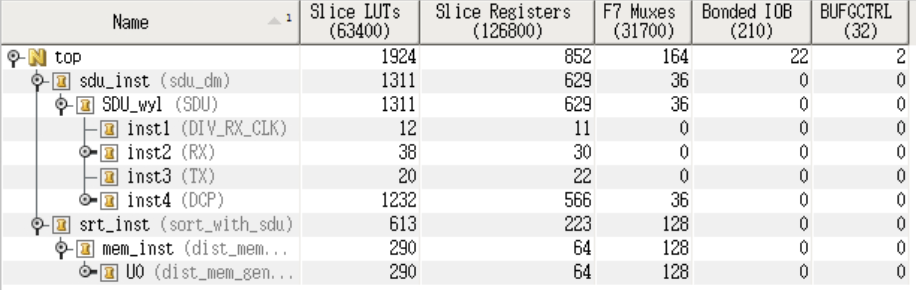
\includegraphics[width=1.0\textwidth]{util.png}
    \caption{Util}
    \label{fig:util}
  \end{figure}


时间性能报告:
\begin{figure}[H]
    \centering
    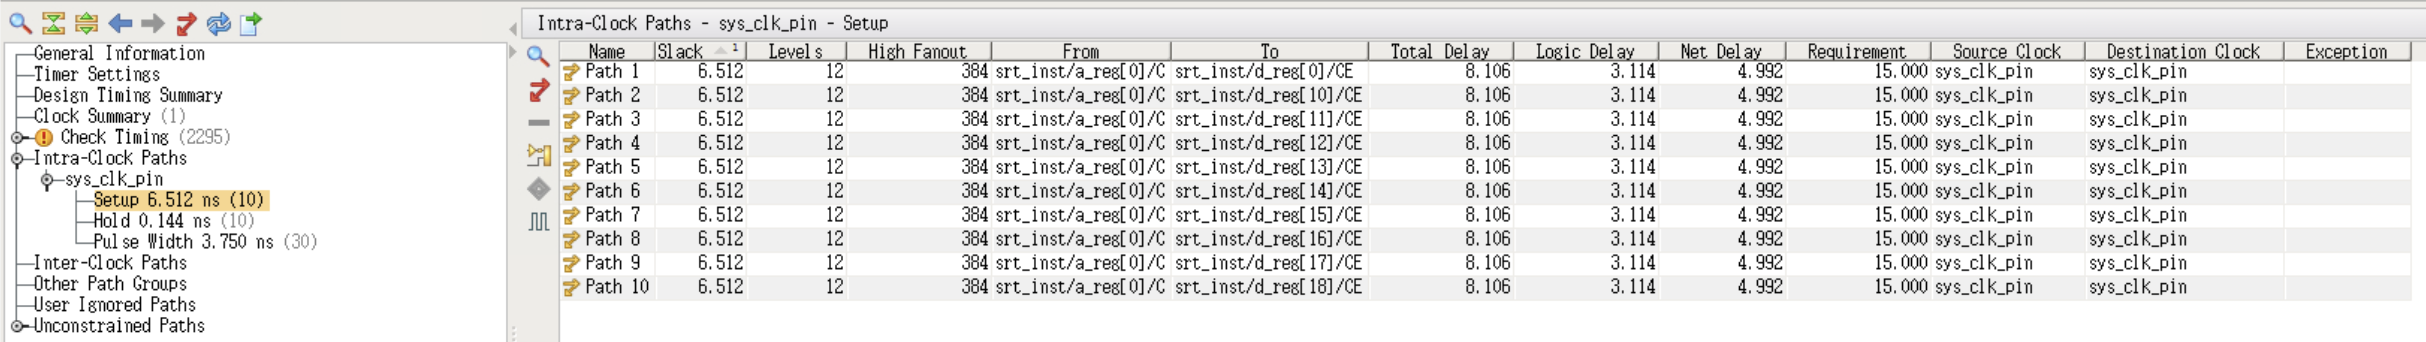
\includegraphics[width=1.0\textwidth]{time.png}
    \caption{time}
    \label{fig:time}
  \end{figure}


\section {实验总结}
\begin{enumerate}
  \item 通过本次实验,我学习了如何使用串口与开发板进行通信,了解了用SDU的调试方法。
  \item 对存储器的设计、结构、读写顺序有了更深刻的认识。
  \item 我学会了如何从高级语言中的循环出发去设计合理的有限状态机。
  \item 学习了查看错误信息来排查bug的方法,提高了调试程序效率。
\end{enumerate}
\section {意见/建议}
大部分调试时间耗费在编写bitstream上,希望可以增加机房开放时间以供调试。
\end{document}